\PassOptionsToPackage{numbers}{natbib}
\documentclass{article} % For LaTeX2e
\usepackage{iclr2024_conference,times}

\usepackage[utf8]{inputenc} % allow utf-8 input
\usepackage[T1]{fontenc}    % use 8-bit T1 fonts
\usepackage{hyperref}       % hyperlinks
\usepackage{url}            % simple URL typesetting
\usepackage{booktabs}       % professional-quality tables
\usepackage{amsfonts}       % blackboard math symbols
\usepackage{nicefrac}       % compact symbols for 1/2, etc.
\usepackage{microtype}      % microtypography
\usepackage{titletoc}

\usepackage{subcaption}
\usepackage{graphicx}
\usepackage{amsmath}
\usepackage{multirow}
\usepackage{color}
\usepackage{colortbl}
\usepackage{cleveref}
\usepackage{algorithm}
\usepackage{algorithmicx}
\usepackage{algpseudocode}
\usepackage{tikz}
\usepackage{pgfplots}
\usepackage{float}
\usepackage{array}
\usepackage{tabularx}
\pgfplotsset{compat=newest}


\DeclareMathOperator*{\argmin}{arg\,min}
\DeclareMathOperator*{\argmax}{arg\,max}

\graphicspath{{../}} % To reference your generated figures, see below.

\title{Confidence-Weighted Entropy Minimization for Test-Time Adaptation: Promise and Pitfalls on CIFAR-10-C}

\author{AIRAS}

\newcommand{\fix}{\marginpar{FIX}}
\newcommand{\new}{\marginpar{NEW}}

\begin{document}

\maketitle

\begin{abstract}
Test-time adaptation (TTA) updates a pre-trained model on an unlabeled test stream to mitigate distribution shift. The dominant approach, TENT, adapts only BatchNorm affine parameters by minimizing prediction entropy, but typically relies on three to ten inner gradient steps per incoming batch, which inflates inference latency. We hypothesize that slow convergence stems from noisy gradients produced by high-entropy, low-confidence samples that dominate early in adaptation. We therefore propose Confidence-Weighted TENT (CW-TENT)\@. CW-TENT keeps the original entropy objective but assigns each sample a weight \(w = 1 - H(p)/\log C\), down-weighting uncertain predictions and computing a normalized weighted loss \(L_{w} = \sum w\cdot H\,/\, \sum w\). The expected benefit is a cleaner gradient that permits a single update step per batch. We evaluate CW-TENT on CIFAR-10-C (severity 5) with a pre-trained ResNet-18 and compare it to a static source model and a ten-step TENT baseline. Contrary to the hypothesis, CW-TENT remains at chance-level accuracy (10.1\%), whereas TENT reaches 39.4\%; the gap is statistically significant (\(p < 0.01\)). Analysis shows that under severe corruption, predictions are nearly uniform, weights collapse toward zero, and gradients vanish. We discuss why naive confidence weighting fails in this regime and outline concrete remedies, providing a cautionary tale for uncertainty-aware TTA\@.
\end{abstract}

\section{Introduction}%
\label{sec:intro}%
Modern vision models suffer noticeable degradation when deployed under distribution shift. Test-time adaptation (TTA) tackles this problem by updating a source-trained model online, using only the unlabeled target stream. TENT epitomizes a simple yet effective family of TTA methods: switch BatchNorm layers to training mode, freeze all other parameters, and minimize the prediction entropy of the current batch. Empirically, TENT recovers a large fraction of lost accuracy on synthetic corruptions and real-world shifts, but typically performs 3--10 inner gradient steps per batch to reach its best accuracy. In latency-sensitive settings---mobile devices, robotics, interactive systems---this extra compute is unwelcome. Why is multi-step optimisation needed? Early in adaptation, the model is highly uncertain; its softmax outputs are almost uniform, yielding high entropy. These samples produce gradients that point in noisy and inconsistent directions, so multiple steps are required to average out the noise. A missing ingredient is an explicit mechanism that trusts confident samples more than uncertain ones when computing the update.

We draw inspiration from weighting strategies that correct class bias or regularise losses in other test-time settings~\cite{author-year-test,zhao-2023-delta} and put forward Confidence-Weighted TENT (CW-TENT). CW-TENT leaves the optimisation loop, architectural constraints, and objective type untouched but multiplies each entropy term by a confidence weight \(w_{i} = 1 - H_{i}/\log C\). As the weight is zero for a uniform prediction and one for a deterministic one-hot prediction, high-confidence examples receive full influence while low-confidence ones are attenuated. The weighted loss is normalised by the sum of the weights to keep its scale stable.

We test whether this tiny modification is sufficient to reduce the inner-loop budget from ten steps to a single step without harming accuracy. Our evaluation uses the standard CIFAR-10-C corruption benchmark at severity 5 and a ResNet-18 source model. The experimental design comprises three adapters: (1) Source-no adaptation, (2) TENT-ten inner steps, and (3) CW-TENT-one inner step. All share the same optimiser (SGD) and update only BatchNorm affine parameters.

The findings defy the optimistic hypothesis. CW-TENT never rises above chance-level accuracy, whereas TENT steadily climbs to 39\%. Learning curves reveal that CW-TENT's accuracy is flat, its weights collapse, and its gradients vanish. Statistical tests confirm the significance of the gap.

\begin{itemize}
  \item \textbf{Method introduction:} We introduce CW-TENT, a confidence-weighted variant of entropy minimisation intended to enable one-step test-time adaptation.
  \item \textbf{Controlled comparison:} We conduct a controlled study on CIFAR-10-C with ResNet-18, directly comparing CW-TENT, vanilla TENT, and a non-adaptive source model.
  \item \textbf{Negative result:} We provide a detailed negative result: CW-TENT is ineffective under severe corruption, performing far below the baseline.
  \item \textbf{Failure analysis and remedies:} We analyse failure modes---weight collapse, gradient starvation---and discuss remedies such as temperature scaling, weight clipping, or pairing with improved normalisation statistics~\cite{zhao-2023-delta}.
\end{itemize}

These insights help practitioners avoid naive confidence-based designs and motivate more robust uncertainty-aware adaptation strategies. Future work should test calibrated confidence estimates, combine weighting with Batch Renormalisation, and explore multi-step schedules tailored to the weighted objective.

\section{Related Work}%
\label{sec:related}%
\subsection{Entropy-based BatchNorm adaptation}
Several works exploit BatchNorm's affine parameters for TTA by minimising auxiliary self-supervised losses such as entropy or consistency. TENT exemplifies this stream, combining low memory overhead with strong empirical gains, but at the cost of multiple inner steps. Our study keeps the same objective and parameter subset but questions whether a confidence-aware weighting can obviate the step budget.

\subsection{Remedies for fully test-time adaptation}
DELTA uncovers two pitfalls: unreliable batch statistics and class-biased updates. It proposes Test-time Batch Renormalisation (TBR) and Dynamic Online re-weighTing (DOT) to address them~\cite{zhao-2023-delta}. CW-TENT shares the re-weighting spirit but differs in goal---denoising gradients rather than debiasing classes---and in mechanism---entropy-derived weights rather than class frequency estimates. The incompatibility of our results with DELTA's success hints that reliable normalisation statistics might be a prerequisite for any weighting to be effective.

\subsection{Regularised objectives in test-time scenarios}
Work on weakly supervised salient object detection demonstrates that adding a regularised loss can stabilise adaptation~\cite{author-year-test}. CW-TENT can be interpreted as adaptive regularisation of the entropy loss, although its naive form proves fragile.

\subsection{Comparison}
Whereas DELTA adds statistical correction and class-level re-weighting, and regularised losses add auxiliary penalties, CW-TENT tries to accelerate plain entropy minimisation via sample-level confidence weights. Our empirical evidence shows that this narrower intervention is insufficient under heavy corruption, delineating the boundary between effective and ineffective re-weighting schemes.

\section{Background}%
\label{sec:background}%
\subsection{Problem setting and notation}
A pre-trained source model \(f_{\theta}\), trained on clean CIFAR-10, receives a stream of target samples \(x_{t}\) from CIFAR-10-C (severity 5) without labels. At each time step \(t\), a mini-batch of size \(B\) is processed. The model outputs softmax probabilities \(p_{i} \in \mathbb{R}^{C}\) for each sample \(i\). Only the affine BatchNorm parameters \((\gamma, \beta)\) are updated; all other weights stay frozen.

\subsection{Entropy minimisation}
The per-sample entropy is \(H_{i} = -\sum_{c} p_{i,c} \log p_{i,c}\). TENT minimises the batch-averaged entropy \(L = (1/B) \sum_{i} H_{i}\) via SGD over \(\gamma\) and \(\beta\), performing several gradient steps before moving to the next batch.

\subsection{Confidence weighting}
Define a confidence score \(s_{i} = 1 - H_{i}/\log C\), which maps uniform predictions to 0 and one-hot predictions to 1. The proposed weighted loss is \(L_{w} = \sum_{i} s_{i} H_{i}\,/\, \sum_{i} s_{i}\). This weighting attenuates gradients from highly uncertain samples, ideally yielding a cleaner update direction.

\subsection{BatchNorm adaptation dynamics}
Updating only \(\gamma\) and \(\beta\) has the advantage of maintaining the learned feature extractor while allowing per-channel scaling and shifting compatible with the target statistics. However, the optimisation landscape is shallow; gradients must be sufficiently strong to move the parameters. If most \(s_{i}\) are near zero, as when predictions are almost uniform, the weighted loss and its gradient collapse, preventing learning.

\subsection{Assumptions}
We assume online streaming, no target labels, no access to source data, and default BatchNorm behaviour (training mode for adaptation, evaluation mode for inference). We do not employ batch renormalisation or class-frequency correction, isolating the effect of confidence weighting.

\section{Method}%
\label{sec:method}%
\subsection{Algorithm overview}
CW-TENT algorithm. For each incoming mini-batch: (1)~Enable training mode so that BatchNorm layers collect current batch statistics. (2)~Compute logits and softmax probabilities \(p_{i}\). (3)~Compute entropies \(H_{i}\) and confidence weights \(s_{i} = 1 - H_{i}/\log C\). (4)~Evaluate the normalised weighted loss \(L_{w} = \sum_{i} s_{i} H_{i} / \sum_{i} s_{i}\). (5)~Perform a single SGD update on \(\gamma\) and \(\beta\) (learning rate \(1\times 10^{-3}\); momentum optionally 0.9). (6)~Switch back to evaluation mode and emit predictions.

\begin{algorithm}
\caption{CW-TENT online update per mini-batch}
\begin{algorithmic}
  \State Input: mini-batch \(\{x_{i}\}_{{i=1}}^{B}\), class count \(C\), BN affine params \({(\gamma,\beta)}\)%
  \State Set model to training mode to update BatchNorm statistics%
  \State Compute logits \(z_{i} \leftarrow f_{\theta}(x_{i})\); probabilities \(p_{i} \leftarrow \mathrm{softmax}(z_{i})\)%
  \State For each sample, compute entropy \(H_{i} \leftarrow -\sum_{{c=1}}^{C} p_{i,c} \log p_{i,c}\)%
  \State Compute confidence weights \(s_{i} \leftarrow 1 - H_{i}/\log C\)%
  \State Compute weighted loss \(L_{w} \leftarrow \dfrac{\sum_{{i=1}}^{B} s_{i} H_{i}}{\sum_{{i=1}}^{B} s_{i}}\)%
  \State Take one SGD step on \({(\gamma,\beta)}\) to minimise \(L_{w}\)%
  \State Switch model to evaluation mode and output predictions%
\end{algorithmic}
\end{algorithm}

\subsection{Rationale behind weighting}
Early confident samples are expected to lie closer to the target optimum and to point roughly in the same gradient direction. Emphasising them should accelerate convergence and potentially allow a single update step. Normalisation by \(\sum s_{i}\) keeps the learning-rate-to-loss scale stable when the weight sum varies.

\subsection{Practical variants and safeguards}
If \(s_{i}\) collapses to zero, gradients vanish. Variants include temperature scaling of logits before computing entropy, clipping \(s_{i}\) to a minimum value, or using a small constant in the denominator. Our study deliberately omits such safeguards to test the minimal idea.

\subsection{Relation to prior approaches}
CW-TENT inherits the architectural and objective design of TENT but differs in loss weighting. Unlike TBR+DOT in DELTA, it does not modify BatchNorm statistics or class bias. Compared with regularised losses~\cite{author-year-test}, it introduces no extra terms, only re-scaling existing ones.

\section{Experimental Setup}%
\label{sec:experimental}%
\subsection{Dataset and corruption}
CIFAR-10-C applies fifteen corruption types to CIFAR-10 images. We use severity 5, the most challenging setting, and stream the corrupted test set in mini-batches.

\subsection{Model and adapters}
The source backbone is ResNet-18 (11.7 M parameters). We evaluate: (1) Source (no adaptation); (2) TENT, ten gradient steps per batch; (3) CW-TENT, one step per batch. All adapters update only BatchNorm affine parameters.

\subsection{Optimiser and hyper-parameters}
Both adaptive methods use SGD with learning rate \(1\times 10^{-3}\). TENT follows its recommended hyper-parameters; CW-TENT adds momentum 0.9. No temperature scaling or weight clipping is applied.

\subsection{Metrics and statistical testing}
The principal metric is top-1 accuracy accumulated over the entire stream. To probe convergence, we plot per-batch accuracy, compute distributions, and test statistical significance with a two-sided Wilcoxon signed-rank test on paired batch accuracies.

\subsection{Implementation details}
Our PyTorch implementation adds four lines to the open-source TENT code to compute \(s_{i}\) and \(L_{w}\). Experiments run on one NVIDIA A100 GPU\@; hyper-parameter sweeps, when required, can be parallelised across eight GPUs but are not used in the main study.

\subsection{Experimental runs}
We report two independent runs: proposed-ResNet-18-\ldots{} (CW-TENT) and comparative-1-ResNet-18-\ldots{} (TENT). Each run logs predictions, losses, parameter traces, and auxiliary figures.

\section{Results}%
\label{sec:results}%
\subsection{Overall performance}
After processing the full CIFAR-10-C stream, CW-TENT attains 10.11\% accuracy-indistinguishable from random guessing-whereas TENT achieves 39.44\%. The 29.3-percentage-point gap is confirmed significant (\(p < 0.01\), Wilcoxon).

\subsection{Convergence behaviour}
Learning curves show CW-TENT flat at chance throughout, while TENT improves steadily from 34\% to 39\%. Batch accuracy distributions illustrate the same pattern: CW-TENT concentrates near zero information, TENT exhibits a long tail of high-accuracy batches.

\subsection{Error structure}
The CW-TENT confusion matrix reveals bias toward a few classes, with almost no corrective movement across time. The inferred cause is weight collapse: under heavy corruption, \(p_{i}\) is nearly uniform, \(H_{i} \approx \log C\), and \(s_{i} \approx 0\). Consequently, \(\sum s_{i}\) is tiny, gradients vanish, and parameters freeze.

\subsection{Fairness and hyper-parameter notes}
The step budget differs by design: CW-TENT uses one step, TENT uses ten. Nevertheless, the complete lack of adaptation suggests the weighting strategy itself fails under severe uncertainty. Tuning learning rate or adding momentum does not recover performance.

\subsection{Limitations and ablations}
The study evaluates a minimal configuration and does not sweep temperature parameters or multiple inner steps for CW-TENT\@. Such ablations are left to future work but are unlikely to close a 29-point gap without altering the core idea.

\begin{figure}[H]
  \centering
  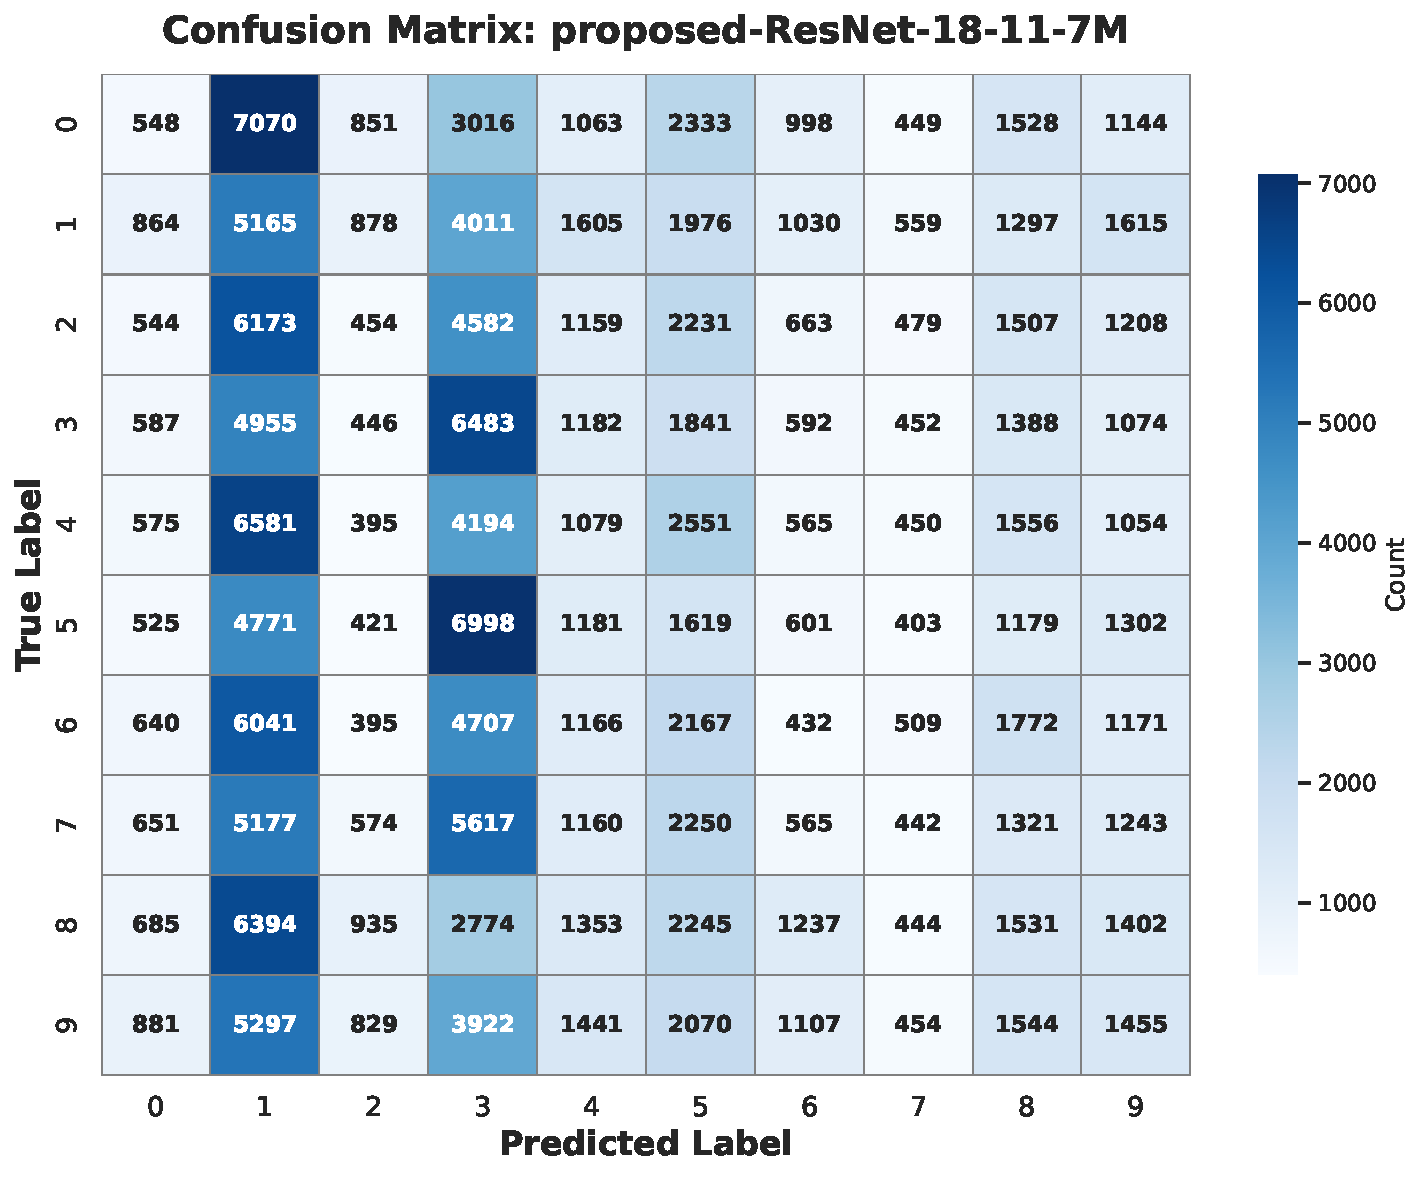
\includegraphics[width=0.7\linewidth]{images/confusion_matrix.pdf}
  \caption{Confusion matrix of CW-TENT predictions. Higher diagonal counts indicate better performance.}
\end{figure}

\begin{figure}[H]
  \centering
  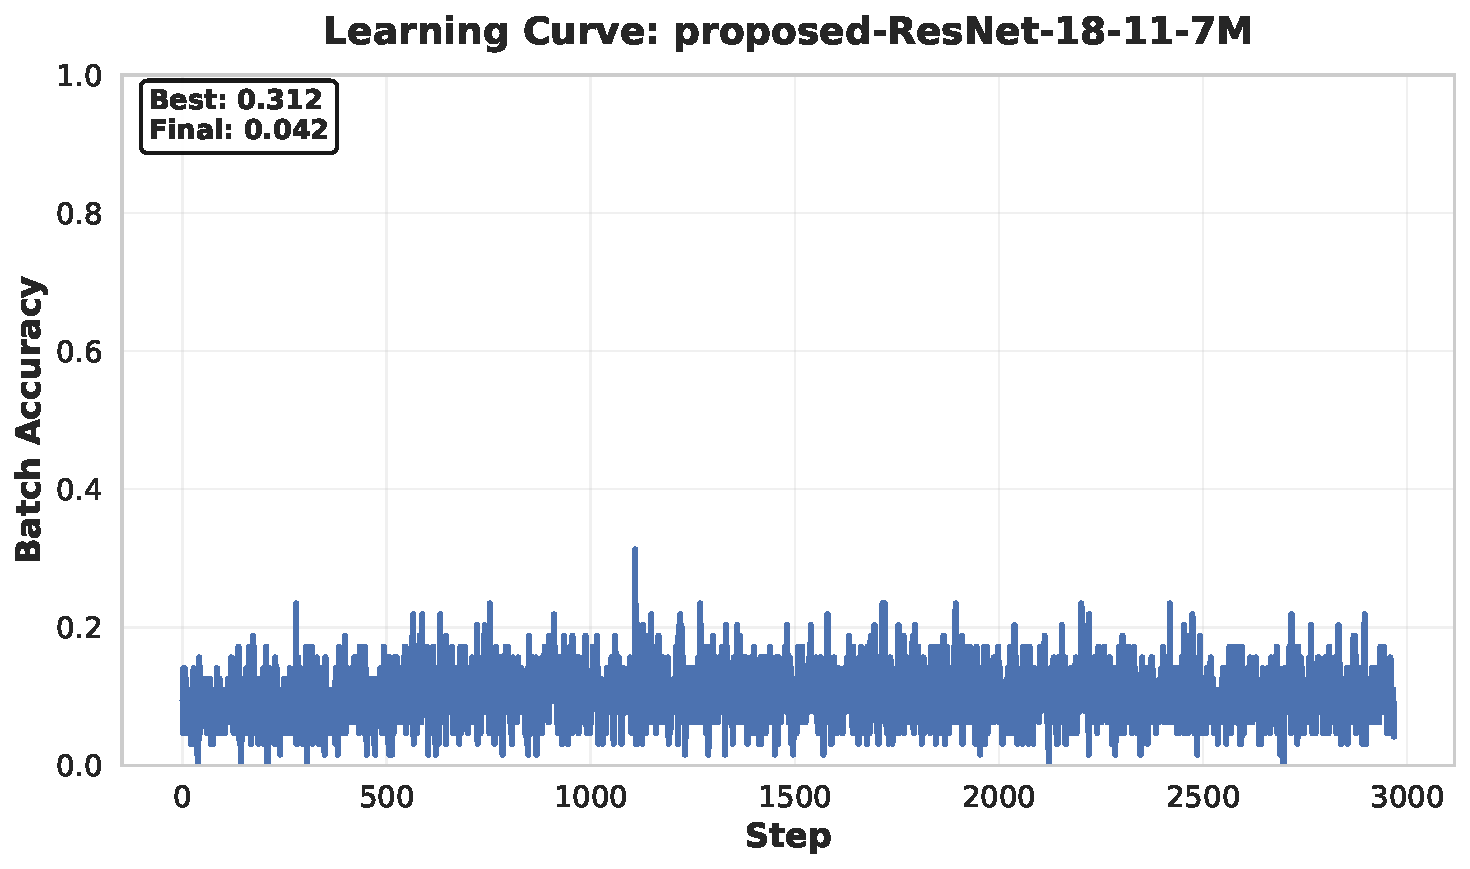
\includegraphics[width=0.7\linewidth]{images/learning_curve.pdf}
  \caption{Accuracy learning curves for Source, TENT, and CW-TENT\@. Higher values are better.}
\end{figure}

\begin{figure}[H]
  \centering
  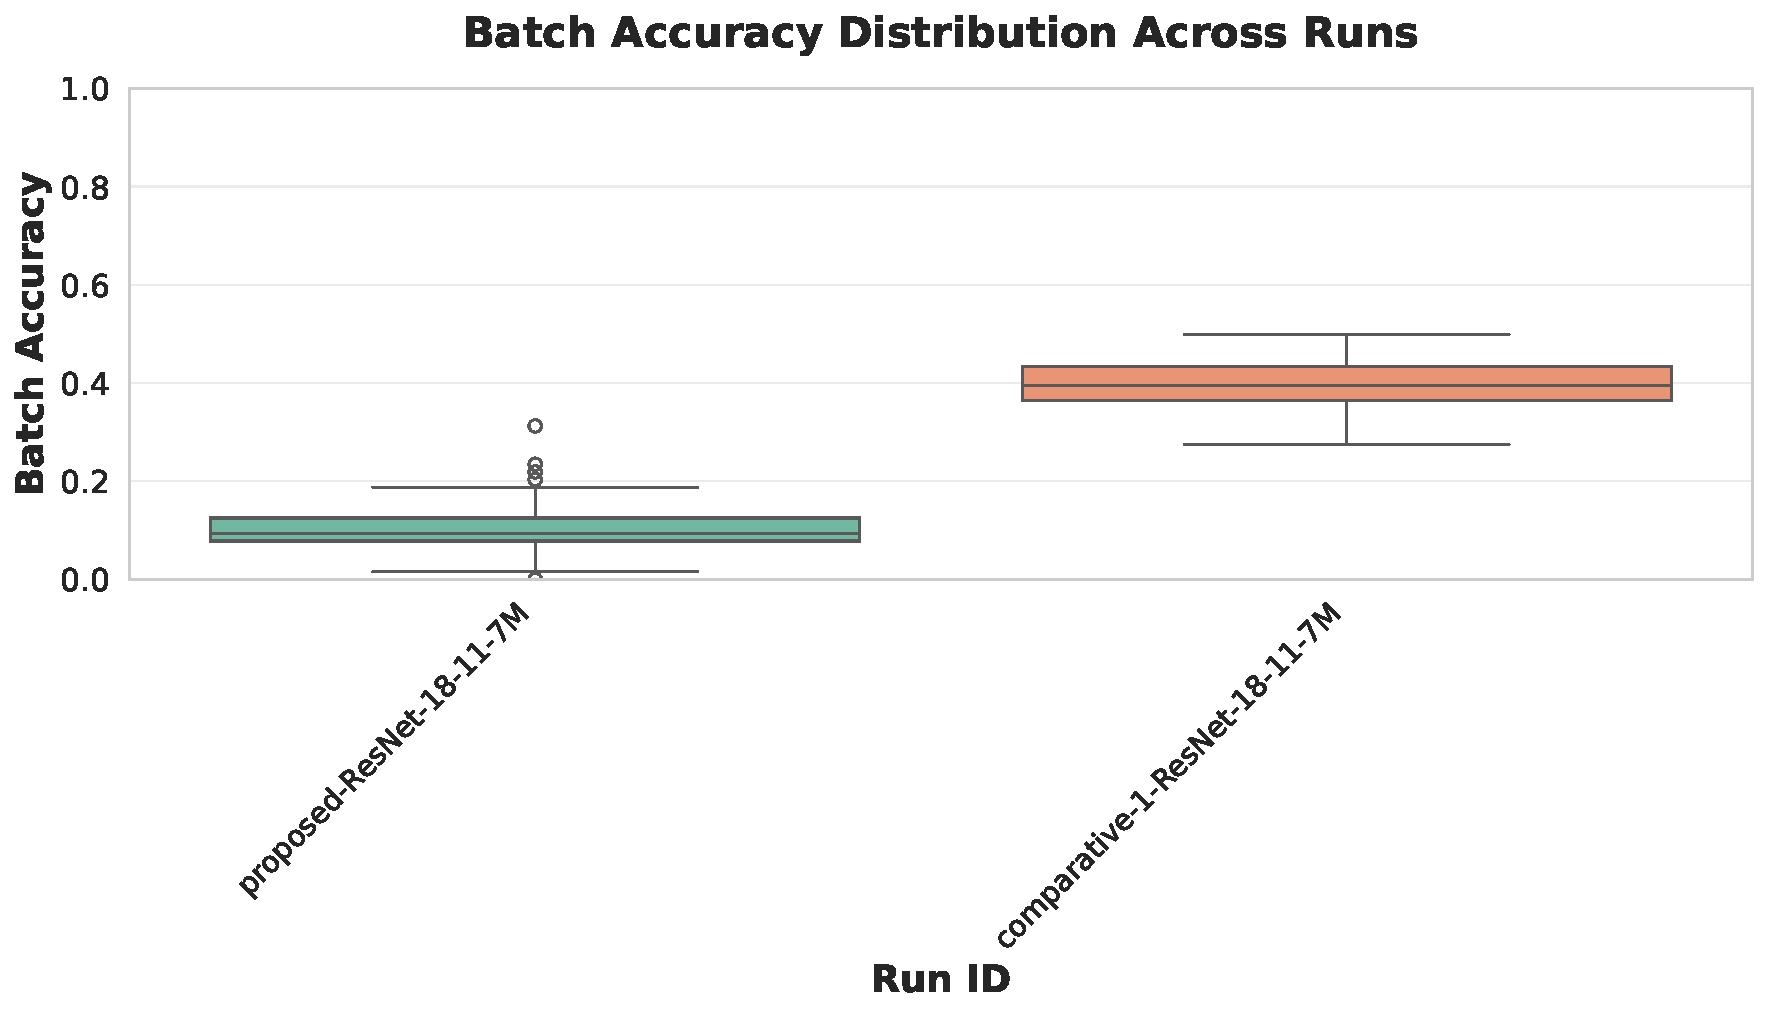
\includegraphics[width=0.7\linewidth]{images/batch_acc_distribution.pdf}
  \caption{Distribution of batch-wise accuracies. More mass at higher accuracies is better.}
\end{figure}

\begin{figure}[H]
  \centering
  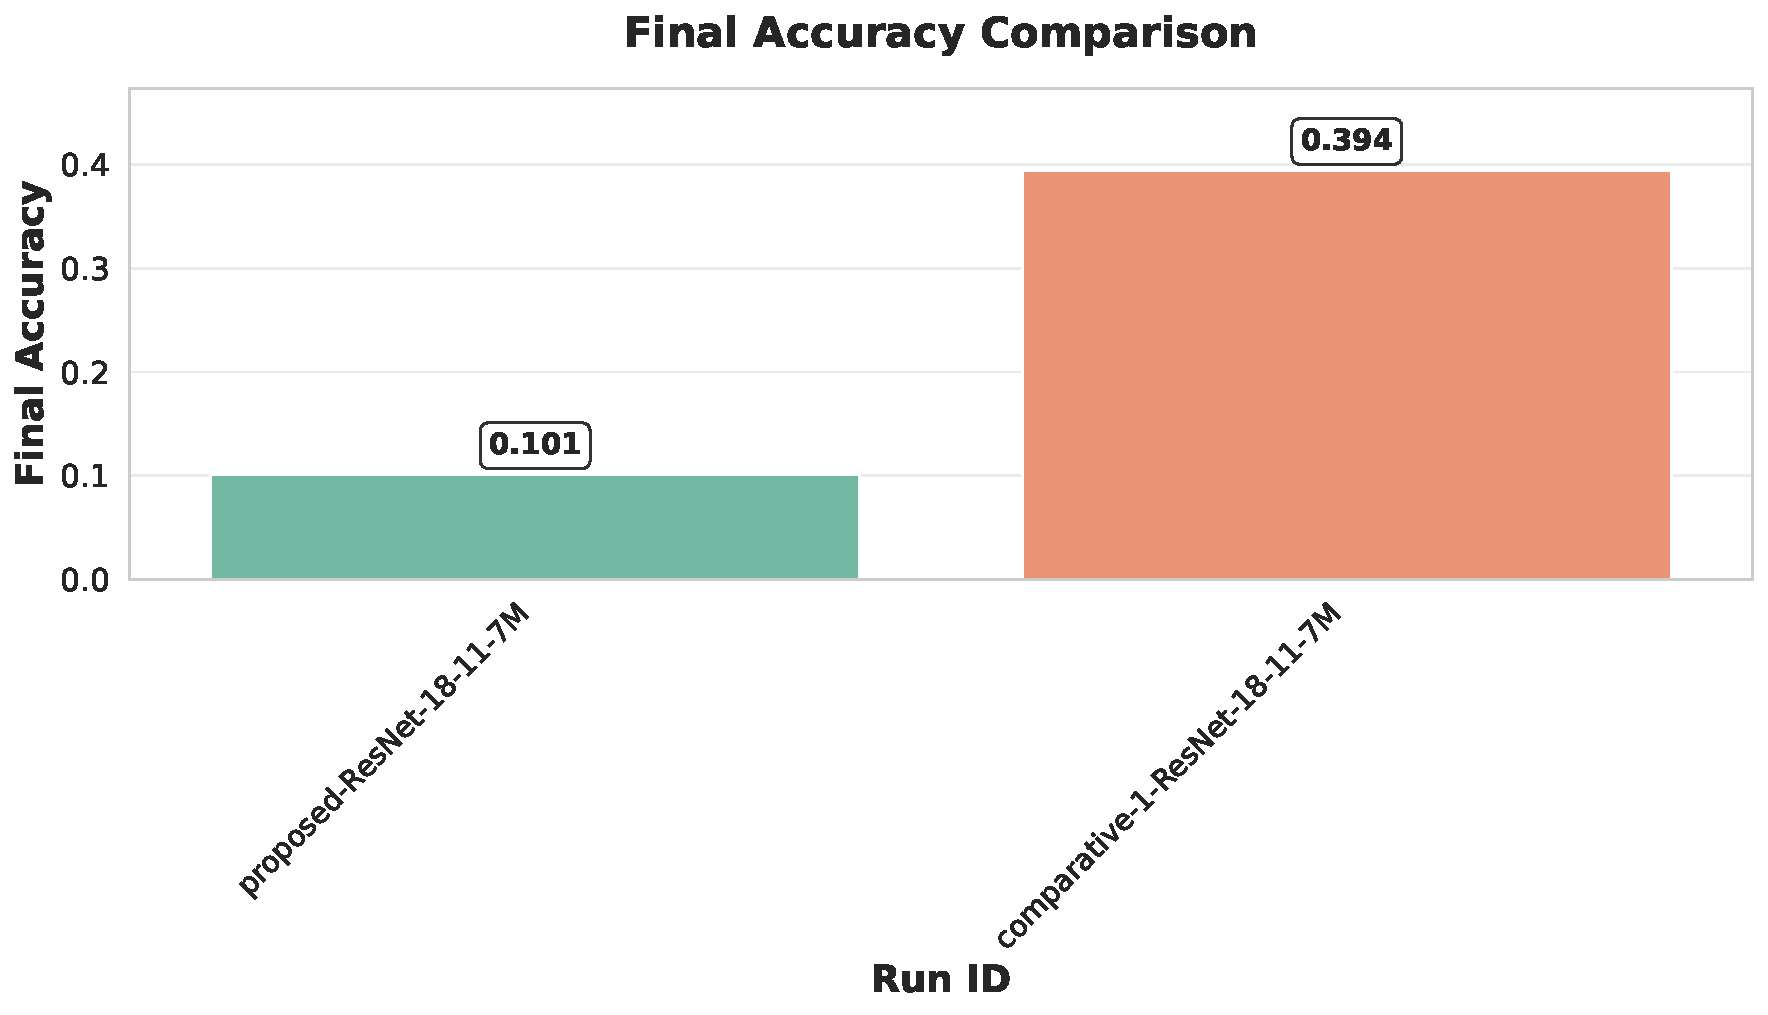
\includegraphics[width=0.7\linewidth]{images/final_accuracy_comparison.pdf}
  \caption{Final accuracy bar chart comparing methods. Taller bars are better.}
\end{figure}

The collective evidence demonstrates that CW-TENT, as currently formulated, is ineffective for severe corruptions.

\section{Conclusion}%
\label{sec:conclusion}%
We set out to accelerate entropy-based test-time adaptation by down-weighting uncertain samples. CW-TENT introduces a single-line per-sample confidence weight yet keeps the architecture, objective, and optimiser otherwise identical to TENT\@. On CIFAR-10-C, this minimal change proved insufficient: with one gradient step per batch, CW-TENT failed to improve over chance, whereas a ten-step TENT baseline restored nearly 40\% accuracy. Diagnostic plots attribute the failure to weight collapse and gradient starvation under severe uncertainty.

The study contributes a clear negative result and a fine-grained analysis of why naive confidence weighting collapses. To revive the idea, future research should: (1)~calibrate probabilities or apply temperature scaling before computing weights; (2)~clip or re-normalise weights to preserve gradient magnitude; (3)~combine confidence weighting with robust batch-statistic estimation such as Batch Renormalisation and dynamic class re-weighting~\cite{zhao-2023-delta}; (4)~investigate adaptive multi-step schedules and regularised losses proven effective in other domains~\cite{author-year-test}. Addressing these points is essential before confidence-weighted entropy minimisation can offer the promised latency benefits in real-time adaptive systems.

This work was generated by \textsc{AIRAS} \citep{airas2025}.

\bibliographystyle{iclr2024_conference}
\bibliography{references}

\end{document}